\chapter{Results}\label{cha:results}

In this chapter, the results of the experiments are reported, as described in \Cref{cha:methods}.


\section{Dataset Generation}

Problem instances are generated as described in \Cref{ssec:probleminstances}. In total, $10000$ training instances, $2000$ validation instances and $ 100 $ test instances of size $100 \times 500$, $200 \times 1000$ and $300 \times 1500$ are created. This is shown in \Cref{tab:instances}.

The generated problem instances are then solved as specified in \Cref{ssec:expertsolutiongeneration}. This results in a total of $162293$ training samples, i.e. nodes with the corresponding evaluation of candidate variables, and $30008$ validation samples. 

\begin{scriptsize}
\begin{table}[ht]
	\centering
	\begin{tabular}{lccccc}
		\toprule
		  Data set& \multicolumn{1}{c}{Train} & \multicolumn{1}{c}{Validate} & \multicolumn{3}{c}{Test}\\ \cmidrule(lr){2-2} \cmidrule(lr){3-3} \cmidrule(lr){4-6}
		  Dimensions & $100 \times 500$ & $100 \times 500$ & $100 \times 500$ & $200 \times 1000$ & $300 \times 1500$ \\
		\addlinespace
		% \midrule
		Instances & 10000 &  2000  & 100 & 20 & 20 \\
		% \addlinespace
		\bottomrule
	\end{tabular}
	\caption{Data set, dimensions and number of problem instances}\label{tab:instances}
\end{table}
\end{scriptsize}

\section{Training}

The training was performed as described in \Cref{sec:trainingprotocol}. 
The training graph for MLP3 is shown in \Cref{fig:training}. The Training and validation loss quickly converges before flattening out. There is no discernible difference between training and validation loss. Loss graphs for MLP1 and MLP2 are not shown, as they are very similar to MLP3's, and are therefore not of interest. 
%
\begin{figure}[h]
    \centering
    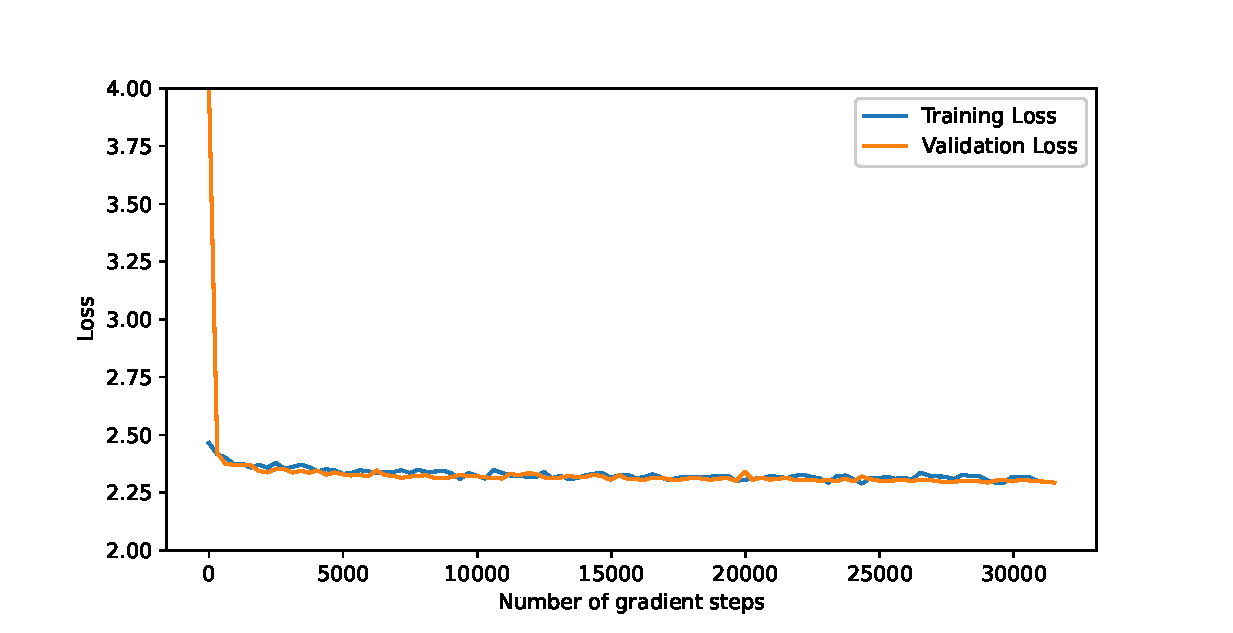
\includegraphics[width=\textwidth]{img/loss70.eps}
    \caption{Training graph for MLP3.}
    \label{fig:training}
\end{figure}


\section{Accuracy}

The top-k accuracy scores for the three \gls{MLP}s along with the benchmark accuracy for random variable selection is shown in \Cref{fig:topk}. Top k accuracy is defined as the number of selected branching variables within the top k variables as determined by the Strong Branching evaluation. 
% https://scikit-learn.org/dev/modules/model_evaluation.html#top-k-accuracy-score

MLP2 and MLP3 show near-identical accuracy, with MLP3 consistently outperformed by 2 - 3 \% at each category. Comparison with the random variable selection policy shows a considerable improvement in favor of the trained models. 

\begin{figure}
    \begin{tikzpicture}
      \begin{axis}[
        mlineplot,
        ylabel={Accuracy [\%]},
        xlabel={Top k},
        width=\textwidth,
        height=7cm,
	    ymin=0.0,   ymax=1.0,
	    xtick=data,
	    legend style={at={(0.01,0.9)},anchor=west}
      ]
        \addplot plot coordinates{(1, 0.413) (2, 0.538) (3, 0.621) (4, 0.681) (5, 0.732) (6, 0.770) (7, 0.800) (8, 0.827) (9, 0.849) (10, 0.867)};
        \addplot plot coordinates{(1, 0.437) (2, 0.568) (3, 0.653) (4, 0.717) (5, 0.767) (6, 0.805) (7, 0.835) (8, 0.860) (9, 0.881) (10, 0.899)};
        \addplot plot coordinates{(1, 0.435) (2, 0.568) (3, 0.652) (4, 0.716) (5, 0.765) (6, 0.802) (7, 0.831) (8, 0.858) (9, 0.879) (10, 0.897)};
        \addplot+ plot coordinates{(1, 0.019) (2, 0.034) (3, 0.047) (4, 0.060) (5, 0.071) (6, 0.081) (7, 0.090) (8, 0.098) (9, 0.107) (10, 0.115)};
        %\addplot+[samples=100] {sin(deg(2*x))};
        \legend{MLP1,MLP2,MLP3,Random}
        
      \end{axis}
    \end{tikzpicture}
    \caption{Top k accuracy of trained models and random variable selection on test set. MLP2 and MLP3 nearly indistinguishable.}
    \label{fig:topk}
\end{figure}
% 0 0.0 acc@1: 43.7 acc@2: 56.8 acc@3: 65.4 acc@4: 71.7 acc@5: 76.6 acc@6: 80.3 acc@7: 83.3 acc@8: 85.9 acc@9: 88.0 acc@10: 89.9

% 61 acc@0:  0.0 acc@1: 41.3 acc@2: 53.8 acc@3: 62.1 acc@4: 68.1 acc@5: 73.2 acc@6: 77.0 acc@7: 80.0 acc@8: 82.7 acc@9: 84.9 acc@10: 86.7

% 70 acc@0:  0.0 acc@1: 43.5 acc@2: 56.8 acc@3: 65.2 acc@4: 71.6 acc@5: 76.5 acc@6: 80.2 acc@7: 83.1 acc@8: 85.8 acc@9: 87.9 acc@10: 89.7


\section{Efficiency}

Five branching strategies were compared on the problem data set of three different problem sizes. The branching strategies are Full Strong Branching, Reliability Pseudo-cost branching, and the three \gls{MLP} topologies. The results are shown in \Cref{tab:results1}. \textit{Time} is the mean solution time, \textit{nodes} is the mean number of nodes in the solution graphs (calculated in accordance with the findings of Gamrath et al. \cite{gamrath2018measuring}), \textit{completed} is the number of problems where optimality was achieved within the time limit of 45 minutes and is only applicable for the large problem size. The branching strategy with the shortest mean solution time is marked bold for each problem size. 

The low-capacity MLP1 branching strategy clearly wins for small problem sizes and is slightly better for medium problem sizes. For large problem sizes, Reliability Pseudo-cost Branching is decisively better, with less than half the solution time of the \gls{MLP} strategies. 

Full Strong Branching results in solution trees orders of magnitude smaller than the \gls{MLP} counterpart. MLP1 is consistently performing faster branching than the other strategies, with respectively $8 \%, 23 \%, 48 \%$ more nodes processed than MLP2 for the three problem sizes.

\Cref{fig:barplot} shows the results for the small problem size from \Cref{tab:results1}, including $95 \%$ confidence intervals.
% \usepackage{booktabs}
 
  
\begin{scriptsize}
\begin{table}[ht]
	\centering
	\begin{tabular}{lrrrrrrr}
		\toprule
		& \multicolumn{2}{c}{Small} & \multicolumn{2}{c}{Medium} & \multicolumn{3}{c}{Large}\\ \cmidrule(lr){2-3} \cmidrule(lr){4-5} \cmidrule(lr){6-8}
		Model & Time (s) & Nodes  & Time (s) & Nodes & Time (s) & Nodes & Completed\\
		\midrule
		FSB & 5.4 &  9.7  & 135.9 &  89.4 & 2070.8 &  520.0 & 12 / 20\\
		PC &  2.5 & 378.3  &  27.3 &  3844.8 & 420.6 &  40130.6 & 20 / 20 \\
		RPC &  3.7 & 27.8  &  22.7 &  987.4 & \textbf{250.1} &  15164.4 & 20 / 20 \\
		\addlinespace
		MLP1 & \textbf{2.1} & 128.6 & \textbf{22.4} & 1224.4 & 606.4 & 22849.8 & 18 / 20\\
		MLP2 & 2.3          & 118.6 & 23.6          & 992.2 & 524.4 & 15408.4  & 18 / 20\\
		MLP3 & 3.0          & 120.2 & 51.2          & 1050.6 & 680.7 & 9889.6  & 15 / 20\\
		\bottomrule
	\end{tabular}
	\caption{Setcover.}\label{tab:results1_set}
\end{table}
\begin{table}[ht]
	\centering
	\begin{tabular}{lrrrrrrr}
		\toprule
		& \multicolumn{2}{c}{Small} & \multicolumn{2}{c}{Medium} & \multicolumn{3}{c}{Large}\\ \cmidrule(lr){2-3} \cmidrule(lr){4-5} \cmidrule(lr){6-8}
		Model & Time (s) & Nodes  & Time (s) & Nodes & Time (s) & Nodes & Completed\\
		\midrule
		FSB & 5.4 &  9.7  & 135.9 &  89.4 & 2070.8 &  520.0 & 12 / 20\\
		PC &  2.5 & 378.3  &  27.3 &  3844.8 & 420.6 &  40130.6 & 20 / 20 \\
		RPC &  3.7 & 27.8  &  22.7 &  987.4 & \textbf{250.1} &  15164.4 & 20 / 20 \\
		\addlinespace
		MLP1 & \textbf{2.1} & 128.6 & \textbf{22.4} & 1224.4 & 606.4 & 22849.8 & 18 / 20\\
		MLP2 & 2.3          & 118.6 & 23.6          & 992.2 & 524.4 & 15408.4  & 18 / 20\\
		MLP3 & 3.0          & 120.2 & 51.2          & 1050.6 & 680.7 & 9889.6  & 15 / 20\\
		\bottomrule
	\end{tabular}
	\caption{Combinatorial auction.}\label{tab:results1_cauction}
\end{table}
\begin{table}[ht]
	\centering
	\begin{tabular}{lrrrrrrr}
		\toprule
		& \multicolumn{2}{c}{Small} & \multicolumn{2}{c}{Medium} & \multicolumn{3}{c}{Large}\\ \cmidrule(lr){2-3} \cmidrule(lr){4-5} \cmidrule(lr){6-8}
		Model & Time (s) & Nodes  & Time (s) & Nodes & Time (s) & Nodes & Completed\\
		\midrule
		FSB & 5.4 &  9.7  & 135.9 &  89.4 & 2070.8 &  520.0 & 12 / 20\\
		PC &  2.5 & 378.3  &  27.3 &  3844.8 & 420.6 &  40130.6 & 20 / 20 \\
		RPC &  3.7 & 27.8  &  22.7 &  987.4 & \textbf{250.1} &  15164.4 & 20 / 20 \\
		\addlinespace
		MLP1 & \textbf{2.1} & 128.6 & \textbf{22.4} & 1224.4 & 606.4 & 22849.8 & 18 / 20\\
		MLP2 & 2.3          & 118.6 & 23.6          & 992.2 & 524.4 & 15408.4  & 18 / 20\\
		MLP3 & 3.0          & 120.2 & 51.2          & 1050.6 & 680.7 & 9889.6  & 15 / 20\\
		\bottomrule
	\end{tabular}
	\caption{Capacitated Facility Location.}\label{tab:results1_facility}
\end{table}
\begin{table}[ht]
	\centering
	\begin{tabular}{lrrrrrrr}
		\toprule
		& \multicolumn{2}{c}{Small} & \multicolumn{2}{c}{Medium} & \multicolumn{3}{c}{Large}\\ \cmidrule(lr){2-3} \cmidrule(lr){4-5} \cmidrule(lr){6-8}
		Model & Time (s) & Nodes  & Time (s) & Nodes & Time (s) & Nodes & Completed\\
		\midrule
		FSB & 5.4 &  9.7  & 135.9 &  89.4 & 2070.8 &  520.0 & 12 / 20\\
		PC &  2.5 & 378.3  &  27.3 &  3844.8 & 420.6 &  40130.6 & 20 / 20 \\
		RPC &  3.7 & 27.8  &  22.7 &  987.4 & \textbf{250.1} &  15164.4 & 20 / 20 \\
		\addlinespace
		MLP1 & \textbf{2.1} & 128.6 & \textbf{22.4} & 1224.4 & 606.4 & 22849.8 & 18 / 20\\
		MLP2 & 2.3          & 118.6 & 23.6          & 992.2 & 524.4 & 15408.4  & 18 / 20\\
		MLP3 & 3.0          & 120.2 & 51.2          & 1050.6 & 680.7 & 9889.6  & 15 / 20\\
		\bottomrule
	\end{tabular}
	\caption{Maximum Independent Set .}\label{tab:results1_indset}
\end{table}
\end{scriptsize}

\begin{figure}
    \centering
    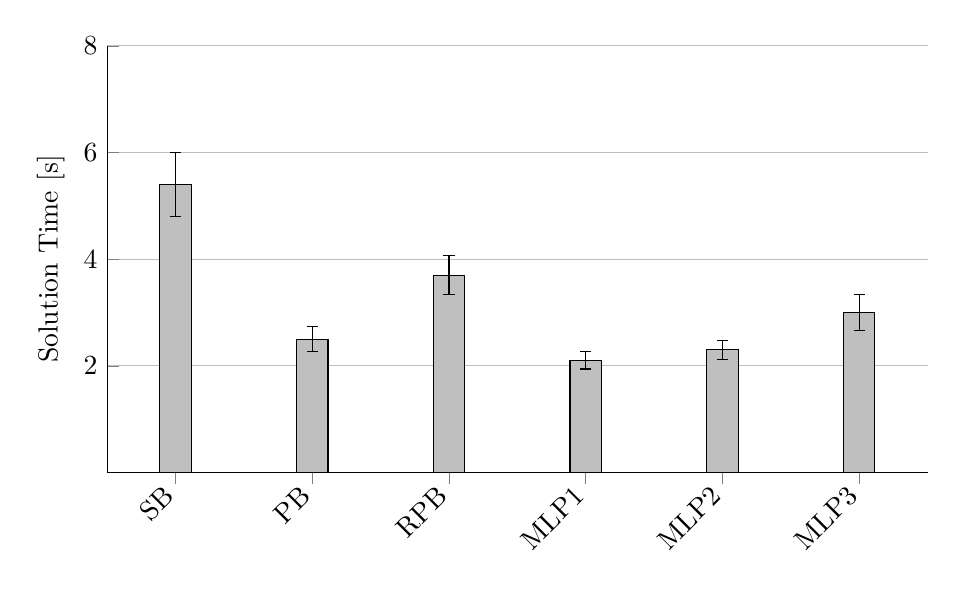
\begin{tikzpicture}
        \begin{axis}[
          width=12cm,
          height=7cm,
          axis x line*=bottom,
          axis y line*=left,
          % nodes near coords,
          legend style={
            at={(0.5,-0.15)},
            anchor=north,
            legend columns=-1
          },
          xtick={1,2,3,4,5,6},
          xticklabels={SB,PB,RPB,MLP1,MLP2,MLP3}, 
          x tick label style={rotate=45,anchor=east},
          ymin=0,
          ymax=8,
          ybar=5pt,
          bar width=0.4cm,
          ylabel={Solution Time [\si{s}]},
          ymajorgrids=true,
          ytick={2,4,...,20}
        ]
          \addplot[color=black,fill=lightgray,error bars/.cd,
    y dir=both,y explicit] coordinates {
            (1,5.4) +- (0.0, 0.6)  %3.27)
            (2,2.5) +- (0.0, 0.24)  %1.2)
            (3,3.7) +- (0.0, 0.37) %1.9)
            (4,2.1) +- (0.0, 0.16) %0.83)
            (5,2.3) +- (0.0, 0.18) %0.93)
            (6,3.0) +- (0.0, 0.33) %1.67)
          };
        \end{axis}
  \end{tikzpicture}
  \caption{Mean solution time with 95 \% confidence intervals for small combinatorial auction problems, n = 100.}
    \label{fig:barplot}
\end{figure}